\documentclass[12pt,a4paper]{article}

% ─── Packages ────────────────────────────────────────────────────────────────
\usepackage[a4paper, margin=1in]{geometry}
\usepackage[T1]{fontenc}
\usepackage{lmodern}
\usepackage{amsmath, amssymb, amsthm}
\usepackage{graphicx}
\usepackage{booktabs}
\usepackage{microtype}
\usepackage{array}
\usepackage{multirow}
\usepackage{xcolor}
\usepackage{caption}
\usepackage{float}
\usepackage{enumitem}
\usepackage{fancyhdr}
\usepackage{titlesec}
\usepackage{abstract}
\usepackage{algorithm}
\usepackage{algpseudocode}
\usepackage{tikz}
\usetikzlibrary{arrows.meta, positioning}
\usepackage{hyperref}

\hypersetup{colorlinks=true, linkcolor=blue!70!black,
            citecolor=green!50!black, urlcolor=blue!70!black}

% ─── Fill these in ───────────────────────────────────────────────────────────
\newcommand{\studentname}{Peeyush Agarwal}
\newcommand{\rollno}{230749}
\newcommand{\department}{Department of Aerospace Engineering}
\newcommand{\supervisor}{Prof.~Urbi Chatterjee}

% ─── Header / Footer ─────────────────────────────────────────────────────────
\setlength{\headheight}{15pt}
\pagestyle{fancy}
\fancyhf{}
\rhead{\small \studentname\ | \rollno}
\lhead{\small UGP Final Report}
\cfoot{\thepage}
\renewcommand{\headrulewidth}{0.4pt}

\titleformat{\section}{\large\bfseries}{\thesection.}{0.5em}{}[\titlerule]
\titleformat{\subsection}{\normalsize\bfseries}{\thesubsection.}{0.5em}{}

\captionsetup{font=small, labelfont=bf}
\setlist{itemsep=2pt, topsep=4pt}
\renewcommand{\arraystretch}{1.12}
\newcommand{\fmt}[1]{\texttt{#1}}
\algrenewcommand\algorithmiccomment[1]{\hfill{\small\color{black!60}$\triangleright$ #1}}

\newtheorem{theorem}{Theorem}
\newtheorem{proposition}{Proposition}
\newtheorem{definition}{Definition}

% ═════════════════════════════════════════════════════════════════════════════
\begin{document}

\begin{titlepage}
    \centering
    \vspace*{1.5cm}
    {\LARGE\bfseries Which Bit Flips Matter?\\[0.4em]
    A Complete Fault-Case Algorithm for\\[0.3em]
    Microscaling (MX) Neural Networks}

    \vspace{1.5cm}
    {\large\textit{Undergraduate Project (UGP) Final Report}}\\[0.3em]
    {\normalsize CS496}

    \vspace{2cm}
    {\large \textbf{\studentname}}\\[0.3em]
    {\normalsize Roll No.: \rollno}\\[0.3em]
    {\normalsize \department}\\[0.3em]
    {\normalsize Indian Institute of Technology Kanpur}

    \vspace{1.5cm}
    {\normalsize Supervisor: \textbf{\supervisor}}\\[0.3em]
    {\normalsize Indian Institute of Technology Kanpur}

    \vspace{2cm}
    {\normalsize November 2026}

    \vfill
    
\includegraphics[width=0.18\textwidth]{iitk_logo.png}
\end{titlepage}

% ─── Abstract ────────────────────────────────────────────────────────────────
\newpage
\begin{abstract}
\noindent
Microscaling (MX) formats store a block of 32 low-precision values together with one shared
8-bit scale. They make inference cheaper, but they also change what a hardware bit flip
does: a flip in an element changes one value, while a flip in the shared scale changes all 32.
A fault-injection campaign tells you \emph{how often} such a network fails. It does not tell
you \emph{which} flips cause the failures, or what would stop them.

This project develops an algorithm that answers that question for every possible single-bit
flip in an MX tensor. A flip becomes a wrong prediction only if five things happen in a row:
the bit really changes, the stored number changes, nothing at read time notices, the datapath
carries the error, and the top-1 answer moves. The algorithm follows this chain. At its core
is a case tree that puts every flip into exactly one of 22 named cases (8 for the scale,
14 for an element). This is checked exhaustively over every code, bit and scale byte of five
formats.

On two exhaustive ResNet8 campaigns (1.1 million injections), the case alone explains 91--97\%
of the variance in damage. Three cases, together 1--2\% of all stored bits, cause more than
half of all failures, and every one of these catastrophic flips is a $0\to1$ flip. Two guards
that follow directly from the algorithm, and need no extra memory, cut the failure rate by
$4.3\times$ (\fmt{e3m2}) and $5.2\times$ (\fmt{e4m3}). A new experiment then uses the
algorithm as a sampling and protection plan on three networks that have no exhaustive
campaign, including a 7-million-parameter RepVGG-A0 and a CIFAR-100 model. With about 1,000
injections it reproduces the exhaustive failure rate of ResNet8 to within 0.2 standard errors,
11--724$\times$ more precisely than uniform sampling of the same size. Its predictions hold on
every network, and on RepVGG-A0 the same guards cut the failure rate by more than two orders of
magnitude.
\end{abstract}

\newpage
\tableofcontents
\newpage

% ═════════════════════════════════════════════════════════════════════════════
\section{Introduction}
% ═════════════════════════════════════════════════════════════════════════════

Deep neural network (DNN) accelerators are moving to narrow number formats, because memory
traffic and arithmetic both get cheaper as the bit width falls. A 4- to 8-bit number cannot
cover the range of a whole weight tensor on its own. \emph{Microscaling} (MX) formats solve this
by grouping values into blocks that share one scale factor~\cite{rouhani2023mx,ocp2023mx}. The
OCP MX specification defines 8-, 6- and 4-bit variants, and they are now supported in commercial
hardware.

Hardware is not fault-free. Radiation strikes, voltage droop and ageing can flip a stored bit,
and in a DNN such a flip can silently change a prediction. This is called silent data corruption
(SDC). DNN reliability under bit flips has been studied for FP32 and integer
formats~\cite{li2017understanding,reagen2018ares,mahmoud2020pytorchfi}. Those studies assume
that each value is its own word, so one flip changes one number. MX breaks that assumption: a
flip in the shared scale changes every value in its block.

The first part of this project (reported earlier) built \texttt{mxfi}, a bit-accurate fault
injector for MX formats, and used it to measure how format, block size, tensor type and bit
position affect the failure rate. That work showed \emph{that} formats with equal accuracy can
differ greatly in reliability. It could not say exactly \emph{which} flips are responsible,
because a campaign returns a single number. To protect a network, a designer needs the
second answer, not the first.

\subsection{Research objective}

\begin{quote}
\textit{Can every single-bit flip in an MX network be sorted, before any injection, into a
small set of cases that predicts its damage, explains why it happens, and tells us how to
stop it?}
\end{quote}

\noindent The goals of this phase were:
\begin{enumerate}
    \item Design a complete and unambiguous classification of single-bit flips in MX tensors,
          covering the scale and the element, and the hardware around them.
    \item Measure each case exactly against exhaustive ground truth, and find out how much of
          the damage the case explains.
    \item Turn the algorithm into something usable: cheap checks and guards that remove the
          dangerous cases, and a sampling plan that cuts the cost of a campaign.
    \item Test whether the algorithm carries over to networks it was not built on.
\end{enumerate}

% ═════════════════════════════════════════════════════════════════════════════
\section{Background}
% ═════════════════════════════════════════════════════════════════════════════

\subsection{Microscaling formats}

An MX block holds $K=32$ values. It is stored as one 8-bit shared exponent $X$ (the
\emph{scale}) and $K$ narrow element codes $m_i$. The value of element $i$ is
\begin{equation}
    v_i = \mathrm{decode}(m_i)\cdot 2^{\,X-127}, \qquad i = 1,\dots,K.
    \label{eq:mx}
\end{equation}
The scale uses the E8M0 encoding: an unsigned power of two, with code 255 reserved for NaN.
Each element is a small sign--exponent--mantissa number. The OCP rule sets
$X = \lfloor \log_2 \max_i |v_i| \rfloor - e_{\max}$, so the largest value of every block lands
in the top binade of the element format. Table~\ref{tab:formats} lists the element formats.

\begin{table}[H]
\centering
\caption{MX element formats. ``Special codes'' are bit patterns that decode to NaN or $\pm\infty$.}
\label{tab:formats}
\small
\begin{tabular}{llccl}
\toprule
\textbf{MX format} & \textbf{Element} & \textbf{Bits (S/E/M)} & \textbf{Largest value} & \textbf{Special codes} \\
\midrule
MXFP8 & \fmt{e4m3} & 1/4/3 & 448    & NaN at \texttt{S.1111.111} \\
MXFP8 & \fmt{e5m2} & 1/5/2 & 57344  & $\pm\infty$, NaN (exp.\ \texttt{11111}) \\
MXFP6 & \fmt{e3m2} & 1/3/2 & 28     & none \\
MXFP6 & \fmt{e2m3} & 1/2/3 & 7.5    & none \\
MXFP4 & \fmt{e2m1} & 1/2/1 & 6      & none \\
\bottomrule
\end{tabular}
\end{table}

\subsection{Two fault sites}

A single-bit flip can land in one of two places:
\begin{itemize}
    \item \textbf{Element flip.} One code $m_i$ changes, so one value changes.
    \item \textbf{Scale flip.} Flipping bit $j$ of $X$ moves the exponent by exactly
          $\Delta = \pm 2^j$, so all $K$ values in the block are multiplied by $2^{\Delta}$.
          Bit 7 gives $\Delta = \pm 128$.
\end{itemize}
Scale bits are only $8/(8+32w)$ of storage for a $w$-bit element (about 4\% for \fmt{e3m2}),
but each one has a blast radius of 32 values.

\subsection{Related work and the gap}

Fault-injection tools such as Ares~\cite{reagen2018ares} and PyTorchFI~\cite{mahmoud2020pytorchfi}
inject random flips and report a failure rate. Statistical fault
injection~\cite{leveugle2009sfi} and value-aware sampling such as TreeFI~\cite{treefi2026} reduce
the number of injections needed to estimate that rate. Bit-flip attacks~\cite{rakin2019bfa,hong2019terminal}
search for the few most damaging bits. None of these gives a \emph{complete, exact} map from a
flip to its effect in MX formats, where the scale and the element interact, and where special
codes, read-time checks and the datapath decide whether a flip is harmless or catastrophic.
That map is what this phase builds.

\subsection{Metric}

Each campaign runs a fixed set of 200 test images. For one fault $f$, the damage is the fraction of
the 200 predictions that change from the fault-free (``golden'') quantised model:
\begin{equation}
    d(f) = \frac{1}{200}\sum_{n=1}^{200} \mathbb{1}\!\left[\hat y_n^{(f)} \neq \hat y_n^{\text{golden}}\right],
    \qquad
    \text{rate} = \mathbb{E}_f\,[d(f)] .
\end{equation}
This is the \emph{per-inference} failure rate: the probability that a random fault changes a
random prediction. An image whose output is NaN or $\infty$ counts as changed. The earlier phase
showed that the more common ``did any image change'' metric depends heavily on which images are
used, so it is not used here.

% ═════════════════════════════════════════════════════════════════════════════
\section{Proposed Methodology: The Flip-Case Algorithm}
% ═════════════════════════════════════════════════════════════════════════════

\subsection{Overview}

A bit flip becomes a wrong answer only if five things all happen (Figure~\ref{fig:chain}). The
algorithm checks them in order, and each stage either stops the fault or passes it on.

\begin{figure}[H]
\centering
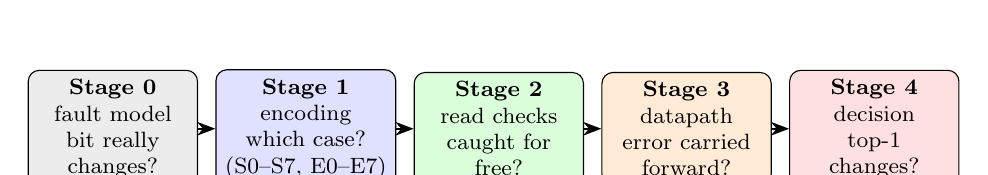
\begin{tikzpicture}[
    box/.style={rectangle, draw, rounded corners, minimum width=2.15cm, minimum height=1.25cm,
                align=center, font=\footnotesize},
    arr/.style={-{Stealth}, thick}]
\node[box, fill=gray!15]  (s0) {\textbf{Stage 0}\\fault model\\bit really\\changes?};
\node[box, fill=blue!12, right=0.22cm of s0] (s1) {\textbf{Stage 1}\\encoding\\which case?\\(S0--S7, E0--E7)};
\node[box, fill=green!14, right=0.22cm of s1] (s2) {\textbf{Stage 2}\\read checks\\caught for\\free?};
\node[box, fill=orange!16, right=0.22cm of s2] (s3) {\textbf{Stage 3}\\datapath\\error carried\\forward?};
\node[box, fill=red!12, right=0.22cm of s3] (s4) {\textbf{Stage 4}\\decision\\top-1\\changes?};
\draw[arr] (s0) -- (s1); \draw[arr] (s1) -- (s2); \draw[arr] (s2) -- (s3); \draw[arr] (s3) -- (s4);
\end{tikzpicture}
\caption{The five-stage chain. A flip that stops at any stage causes no failure. Stage~1 is the
case tree; stages 0, 2 and 3 describe the memory, the reader and the arithmetic around it.}
\label{fig:chain}
\end{figure}

\subsection{Stage 0: the fault model}

A transient flip can go $0\to1$ or $1\to0$. A stuck-at fault only does something when the stored
bit differs from the stuck value. Memory technologies are often asymmetric (for example, DRAM
charge loss is mostly $1\to0$), so the algorithm weights each flip by the probability of its
direction rather than assuming both are equally likely.

\subsection{Stage 1: the case tree}

This is the core of the algorithm. For a scale flip, $X' = X \oplus 2^j$ and
$\Delta = X' - X$. For an element flip, $c' = c \oplus 2^b$ and the value moves from $v$ to
$v'$. The cases are checked in the order of Algorithm~\ref{alg:cases}, and the first match wins.
Tables~\ref{tab:scale} and~\ref{tab:element} give their meaning.

\begin{algorithm}[H]
\caption{Stage 1: the case of one single-bit flip}
\label{alg:cases}
\begin{algorithmic}[1]
\small
\If{the flip hits scale byte $X$, bit $j$}
    \State $X' \gets X \oplus 2^j$; \quad $\Delta \gets X' - X$ \Comment{block scaled by $2^{\Delta}$}
    \If{$X' = 255$} \Return \textbf{S1} to NaN \Comment{whole block NaN}
    \ElsIf{$X = 255$} \Return \textbf{S7} from NaN \Comment{only after an earlier fault}
    \ElsIf{every element is $\pm 0$} \Return \textbf{S0} zero block \Comment{masked}
    \ElsIf{$\Delta = +128$ or block overflows FP32} \Return \textbf{S2} overflow
    \ElsIf{$\Delta \ge 8$} \Return \textbf{S3} grow $\ge 256\times$
    \ElsIf{$\Delta > 0$} \Return \textbf{S4} grow $2$--$16\times$
    \ElsIf{$\Delta \ge -2$} \Return \textbf{S5} shrink $2$--$4\times$
    \Else\ \Return \textbf{S6} erase \Comment{shrink $\ge 16\times$}
    \EndIf
\Else \Comment{element code $c$, bit $b$}
    \State $c' \gets c \oplus 2^b$
    \If{$c$ is NaN/Inf} \Return \textbf{E7} from special
    \ElsIf{$c'$ is NaN/Inf} \Return \textbf{E1} to special
    \ElsIf{$b$ is the sign bit} \Return \textbf{E0} if $v = \pm 0$, else \textbf{E2} negate
    \ElsIf{exponent bit set $0\to1$} \Return \textbf{E3a} from zero / \textbf{E3b} subnormal$\to$normal / \textbf{E3} grow
    \ElsIf{exponent bit cleared} \Return \textbf{E4a} to zero / \textbf{E4b} normal$\to$subnormal / \textbf{E4} shrink
    \ElsIf{mantissa bit set} \Return \textbf{E5a} from zero / \textbf{E5} grow
    \Else\ \Return \textbf{E6a} to zero / \textbf{E6} shrink
    \EndIf
\EndIf
\end{algorithmic}
\end{algorithm}

\begin{table}[H]
\centering
\caption{Scale cases. $P_B$ is the block's partial sum in the next layer.}
\label{tab:scale}
\begin{tabular}{lll}
\toprule
\textbf{Case} & \textbf{Condition} & \textbf{Effect} \\
\midrule
S0 zero block   & all elements $\pm0$              & none (masked) \\
S1 to NaN       & $X' = 255$                       & 32 NaNs \\
S2 overflow     & $\Delta = +128$ or FP32 overflow & $\pm\infty$ when $|P_B|\,2^{\Delta}$ overflows \\
S3 grow large   & $\Delta \ge 8$                   & block $\times 256$ or more \\
S4 grow small   & $\Delta \in \{1,2,4\}$           & block $\times 2$, $\times 4$, $\times 16$ \\
S5 shrink small & $\Delta \in \{-1,-2\}$           & block $\div 2$, $\div 4$ \\
S6 erase        & $\Delta \le -4$                  & block $\div 16$ or more, nearly deleted \\
S7 from NaN     & $X = 255$                        & only after an earlier fault \\
\bottomrule
\end{tabular}
\end{table}

\begin{table}[H]
\centering
\caption{Element cases. Sub-cases mark a change of value class (zero, subnormal, normal).}
\label{tab:element}
\small
\begin{tabular}{lll}
\toprule
\textbf{Case} & \textbf{Field / direction} & \textbf{Effect} \\
\midrule
E0 masked      & sign of $\pm 0$     & none \\
E1 to special  & any bit, into NaN/Inf code & NaN or $\pm\infty$ weight \\
E2 negate      & sign                & $v \to -v$, error $2|v|$ \\
E3 / E3a / E3b & exponent $0\to1$    & grow $\times 2^{2^k}$ / from zero / sub.$\to$normal \\
E4 / E4a / E4b & exponent $1\to0$    & shrink $\div 2^{2^k}$ / to zero / normal$\to$sub. \\
E5 / E5a       & mantissa $0\to1$    & small growth / from zero \\
E6 / E6a       & mantissa $1\to0$    & small shrink / to zero \\
E7 from special& code already NaN/Inf & only after an earlier fault \\
\bottomrule
\end{tabular}
\end{table}

\begin{theorem}[Completeness]
For each of the five element formats, every pair (code, bit) of an element and every pair
(byte $X \in \{0,\dots,255\}$, bit $j$) of a scale, for both zero and non-zero blocks, falls
into exactly one case of Algorithm~\ref{alg:cases}.
\end{theorem}
\begin{proof}[Argument and check]
Inside each branch the conditions are tested in a fixed order and the last branch has no
condition, so every flip gets a case and no flip gets two. Because the input space is finite,
this was also checked by brute force: the test suite enumerates all codes, bits and scale
bytes of all five formats and asserts that each lands in one valid case (38 tests, all passing).
\end{proof}

\noindent The case tree explains the \emph{catastrophic} flips. Call E1, S1 and S2 the
catastrophic cases: they produce NaN or $\infty$ values.

\begin{proposition}[Catastrophic flips are $0\to1$]
Every flip in a catastrophic case sets a bit that was $0$.
\end{proposition}
\begin{proof}
NaN and Inf codes are runs of 1s: \texttt{S.1111.111} in \fmt{e4m3}, exponent \texttt{11111} in
\fmt{e5m2}, and $255 = \texttt{11111111}$ for E8M0. A finite code has at least one 0 in that run,
and a single flip can reach the all-ones pattern only by setting that 0. For S2, $\Delta > 0$, and
$\Delta = X' - X = +2^j$ exactly when bit $j$ was 0.
\end{proof}

\noindent So a memory that mostly loses charge ($1\to0$) cannot produce a catastrophic flip at all,
and a stuck-at-0 bit is almost harmless. Section~\ref{sec:direction} measures this.

\subsection{Stage 2: free checks and guards}

A clean OCP MX tensor obeys invariants that can be checked at read time with \emph{no extra
memory}:
\begin{itemize}
    \item \textbf{D1:} no element code is NaN/Inf (a clean tensor never stores one). If one is
          found, guard \textbf{G1} decodes it as 0, so E1 becomes ``one weight zeroed''.
    \item \textbf{D2:} every scale lies inside the tensor's clean band $[X_{\min}, X_{\max}]$,
          known offline for weights. If a scale is above the band, guard \textbf{G2} treats the
          block as 0, so S1/S2/S3 become an S6-like erase.
    \item \textbf{D3:} every non-zero block has an element in the top binade (the OCP rule
          guarantees it). A block that lost it was hit by a fault.
\end{itemize}

\subsection{Stages 3--5: datapath, decision and use}

Whether a NaN reaches the output depends on the hardware. With IEEE arithmetic NaN survives
every operation, and $\mathrm{NaN}\cdot 0 = \mathrm{NaN}$, so even zero inputs do not mask it.
A ReLU written as \texttt{x > 0 ? x : 0} turns NaN into 0, which erases one output channel
instead. $+\infty$ passes any ReLU, $-\infty$ does not. A finite error reaching the next layer
is about $\delta \cdot a$ for an element (weight error times input activation) and
$(2^{\Delta}-1)\,P_B$ for a scale. At stage 4 the outcome is one of: no change, silent
corruption, or a non-finite output that one \texttt{isfinite} check on the logits catches.
Stage 5 adds up the damage over all faults, weighted by stage 0.

\subsection{Using the algorithm to plan a campaign}
\label{sec:stratified}

Stage 1 needs no injection: the case of every stored bit can be counted exactly from the
quantised weights. Element cases depend only on (code, bit), so a histogram of codes per tensor
is enough. This makes the algorithm a sampling plan. Let stratum $h$ be the set of faults with
case $c$ and direction (bit was 0 or 1), with exact size $N_h$ and weight $W_h = N_h/N$. Then
\begin{equation}
    \widehat{\text{rate}} = \sum_h W_h\, \bar d_h, \qquad
    \widehat{\mathrm{Var}} = \sum_h W_h^2\, \frac{s_h^2}{n_h}\left(1 - \frac{n_h}{N_h}\right),
\end{equation}
where $\bar d_h$ and $s_h^2$ are the mean and variance of the $n_h$ injected faults of stratum
$h$. Masked cases (E0, S0) have damage exactly 0 and are not injected at all. Small strata are
injected completely. The catastrophic strata, which hold most of the damage but very few faults,
are no longer left to chance.

% ═════════════════════════════════════════════════════════════════════════════
\section{Experimental Setup}
% ═════════════════════════════════════════════════════════════════════════════

\subsection{Models and data}

\begin{table}[H]
\centering
\caption{Networks. Accuracy is the MX-quantised accuracy on the 200 campaign images.}
\label{tab:models}
\small
\begin{tabular}{llrll}
\toprule
\textbf{Network} & \textbf{Dataset} & \textbf{Parameters} & \textbf{Used in} & \textbf{Ground truth} \\
\midrule
ResNet8 (width 16)~\cite{he2016resnet,banbury2021mlperftiny} & CIFAR-10  & 78\,K  & E25--E29 & exhaustive \\
ResNet8                   & CIFAR-100 & 85\,K  & E29 & sampled \\
RepVGG-A0~\cite{ding2021repvgg} & CIFAR-10 & 7.0\,M & E28, E29 & sampled \\
\bottomrule
\end{tabular}
\end{table}

\noindent All weights of all convolutional and linear layers are quantised to MX with block size 32
and the OCP scale rule. CIFAR-100 stands in for a harder task, since ImageNet was not available on
the machines used. The two ResNet8 CIFAR-10 networks are the exact checkpoints on which the
exhaustive campaigns were recorded (one for \fmt{e3m2}, one for \fmt{e4m3}).

\subsection{Experiments}

\begin{table}[H]
\centering
\caption{Experiments of this phase.}
\label{tab:experiments}
\begin{tabular}{p{1.1cm}p{13.2cm}}
\toprule
\textbf{ID} & \textbf{What it does} \\
\midrule
E25 & Labels every fault of the two exhaustive ResNet8 campaigns (483,904 faults for \fmt{e3m2},
      638,624 for \fmt{e4m3}) with its case, so each case gets its exact damage. \\
E26 & Re-injects the catastrophic cases under a NaN-zeroing ReLU and under guard G1. \\
E27 & Stage 0 and 2: flip direction, checks D1--D3 and guards, held-out variance explained, protection order. \\
E28 & Activations: case mix, scale-band checks, and how re-quantisation spreads an error (exact counting, no injection). \\
E29 & \textbf{New:} the algorithm as a sampling and protection plan on three networks (Section~\ref{sec:e29}). \\
\bottomrule
\end{tabular}
\end{table}

\noindent E25, E27 and E28 were re-run for this report and reproduced the earlier outputs exactly.
E29 injects 60 faults per stratum on the ResNet8 networks and 25 on RepVGG-A0, and scores each
fault three times: with no protection, with guards G1+G2, and with a NaN-zeroing ReLU. Everything ran on
a 4-core laptop CPU, except the two exhaustive campaigns, which ran earlier on the IIT Kanpur GPU
cluster.

% ═════════════════════════════════════════════════════════════════════════════
\section{Results and Analysis}
% ═════════════════════════════════════════════════════════════════════════════

\subsection{A few cases hold most of the damage}

\begin{figure}[H]
\centering
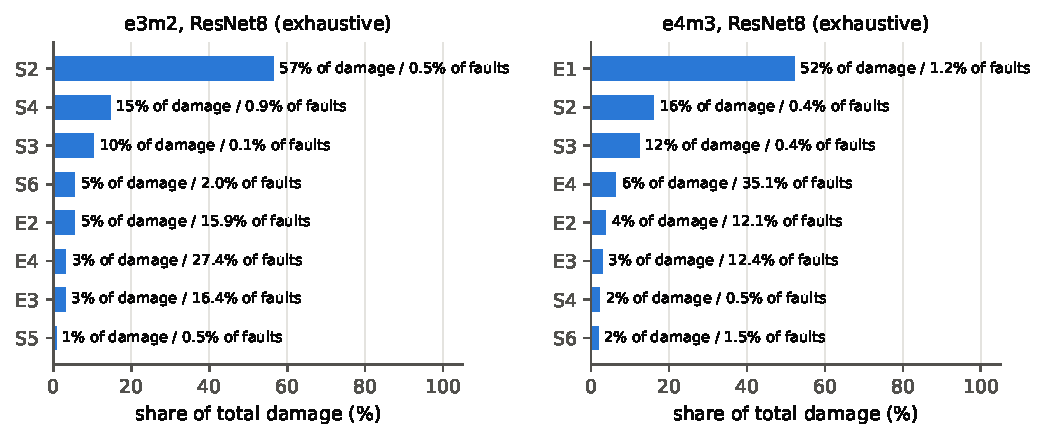
\includegraphics[width=\textwidth]{fig/case_damage.pdf}
\caption{Share of total damage per case on the exhaustive ResNet8 campaigns (top 8 cases).
Each bar is labelled with its share of damage and its share of all faults.}
\label{fig:cases}
\end{figure}

Figure~\ref{fig:cases} shows the main pattern. In \fmt{e3m2}, the S2 scale overflow is 0.5\% of
all faults and causes 57\% of all damage (mean damage 0.97: almost every image fails). In
\fmt{e4m3}, flips into a NaN code (E1) are 1.2\% of faults and cause 52\% of damage, with damage
exactly 1.0 for every one of them. The common element cases (E2--E6) are 80--95\% of faults but
only 9--16\% of damage.

The case explains the catastrophic part almost completely, but not the small finite errors
(Table~\ref{tab:r2}). Within ordinary element flips the case explains only 2--5\%; what matters
there is the size of the error that reaches the next layer, $|v'-v|\cdot 2^{X-127}$ times the
input activity. That raises the explained variance to 64--67\%.

\begin{table}[H]
\centering
\caption{Held-out variance of damage explained ($R^2$, two-fold), adding one factor at a time.}
\label{tab:r2}
\begin{tabular}{lcccc}
\toprule
& \multicolumn{2}{c}{\textbf{All faults}} & \multicolumn{2}{c}{\textbf{Ordinary element flips}} \\
\textbf{Model} & \fmt{e3m2} & \fmt{e4m3} & \fmt{e3m2} & \fmt{e4m3} \\
\midrule
Site only (scale or element)   & 0.22 & 0.09 & 0.00 & -- \\
+ case (Algorithm 1)           & \textbf{0.91} & \textbf{0.97} & 0.02 & 0.05 \\
+ bit position and layer       & 0.94 & 0.98 & 0.19 & 0.21 \\
+ error size $\times$ input activity & 0.94 & 0.98 & \textbf{0.67} & \textbf{0.64} \\
\bottomrule
\end{tabular}
\end{table}

\subsection{Flip direction decides the risk}
\label{sec:direction}

\begin{table}[H]
\centering
\caption{Stage 0 on the exhaustive campaigns. ``0$\to$1 only'' is also the rate under stuck-at-1 faults.}
\label{tab:direction}
\begin{tabular}{lcc}
\toprule
& \fmt{e3m2} & \fmt{e4m3} \\
\midrule
Stored bits that are 0                 & 43\%   & 40\% \\
Damage caused by $0\to1$ flips         & 87.5\% & 88.7\% \\
Rate, $0\to1$ flips only               & 0.00768 & 0.02089 \\
Rate, $1\to0$ flips only               & 0.00110 & 0.00267 \\
Ratio                                  & $7.0\times$ & $7.8\times$ \\
Catastrophic faults that are $0\to1$   & 2,468 of 2,468 & 10,321 of 10,321 \\
\bottomrule
\end{tabular}
\end{table}

As Proposition~1 predicts, every catastrophic fault is a $0\to1$ flip. The failure rate is
therefore not a property of the format alone: a memory whose upsets are mostly $1\to0$ would see
about $7$--$8\times$ fewer failures than the usual symmetric fault model assumes.

\subsection{Free checks catch most of the damage}

\begin{table}[H]
\centering
\caption{Stage 2: share of damage flagged by each read-time check, and the rate after the guards.}
\label{tab:guards}
\small
\begin{tabular}{lcc}
\toprule
& \fmt{e3m2} & \fmt{e4m3} \\
\midrule
D1 element code is NaN/Inf               & --     & 52.2\% \\
D2 scale outside its tensor's clean band & 85.7\% & 32.1\% \\
D3 block lost its top-binade element     & 0.1\%  & 0.2\% \\
D1 + D2 + D3 together                    & 85.8\% & 84.5\% \\
\midrule
Rate, no guard                           & 0.00878 & 0.0236 \\
Rate, G1 + G2                            & 0.00206 ($\mathbf{4.3\times}$ lower) & 0.00454 ($\mathbf{5.2\times}$ lower) \\
\bottomrule
\end{tabular}
\end{table}

The three checks flag only 3.5--4.1\% of faults, but those faults carry 85\% of the damage. The
two guards cost no storage, only a comparison at read time. G1 alone cut the damage of an E1
fault from 1.0 to 0.0064 (measured on 2,000 injected E1 faults).

\subsection{The datapath can turn a catastrophic flip into a mild one}

\begin{table}[H]
\centering
\caption{Stage 3: mean damage of the catastrophic cases under three datapaths (E26).}
\label{tab:datapath}
\small
\begin{tabular}{lccc}
\toprule
& \textbf{ReLU passes} & \textbf{ReLU zeroes} & \\
\textbf{Case} & \textbf{NaN} & \textbf{NaN} & \textbf{Read guard} \\
\midrule
E1 element $\to$ NaN, all layers & 1.00 & 0.085 & 0.0064 (G1) \\
E1 element $\to$ NaN, final layer & 1.00 & 1.00 & 0.002--0.02 (G1) \\
S2 scale $+128$, \fmt{e3m2} / \fmt{e4m3} & 0.98 / 0.98 & 0.97 / 0.97 & erased (G2) \\
\bottomrule
\end{tabular}
\end{table}

The same E1 flip is catastrophic or mild depending on one detail of the ReLU. The S2 flip is not
helped by the ReLU, because it usually produces $+\infty$, which passes any ReLU; only a scale
check stops it.

\subsection{Activations and re-quantisation}

Activations differ from weights: 40--55\% of activation values are exactly 0, so a large share of
flips are masked or only turn a 0 into a tiny value. In an all-MX pipeline every activation is
re-quantised, and an error that grows one value raises its block's scale and can flush the other
31 values to 0 (Table~\ref{tab:requant}). This reverses the NaN story: the formats without NaN
codes are the ones whose errors spread.

\begin{table}[H]
\centering
\caption{Share of non-zero neighbours flushed to 0 when the block maximum grows by $r$ (real ResNet8 activations).}
\label{tab:requant}
\begin{tabular}{lccccc}
\toprule
\textbf{Format} & $r=2$ & $r=4$ & $r=16$ & $r=256$ & $r=65536$ \\
\midrule
\fmt{e5m2} & 0 & 0 & 0 & 0 & 0 \\
\fmt{e4m3} & 0 & 0 & 0.01\% & 0.1\% & 29\% \\
\fmt{e3m2} & 0.5\% & 0.9\% & 3.9\% & 55\% & 100\% \\
\fmt{e2m1} & 15\% & 29\% & 91\% & 100\% & 100\% \\
\bottomrule
\end{tabular}
\end{table}

\subsection{New experiment (E29): the algorithm on other networks}
\label{sec:e29}

E25--E28 built the algorithm on one network. E29 asks two practical questions on networks that
have no exhaustive campaign: (1) does the case-stratified estimate of Section~\ref{sec:stratified}
give the right rate with far fewer injections, and (2) do the guards and the direction rule carry
over?

\paragraph{Estimation.} Table~\ref{tab:e29est} shows the case-stratified estimate. On the two ResNet8
networks, where the exhaustive answer is known, about 1,000 injections give the exhaustive rate
to within 0.2 standard errors. An exhaustive campaign needed 484--639 thousand. Compared with
uniform sampling of the same size, the variance is $11$--$724\times$ smaller. Put another way, a
uniform campaign would need that many times more injections for the same precision. The RepVGG-A0
fault space has 44--58 million bits, so an exhaustive campaign is out of reach there. The algorithm
needs 425--450 injections, and most of them only confirm that the ordinary cases do almost nothing.

\begin{table}[H]
\centering
\caption{E29 estimation. ``Faults'' is the exact size of the fault space, counted by the
algorithm without injection. Rate is mean $\pm$ one standard error. Variance reduction is
against a uniform campaign with the same number of injections.}
\label{tab:e29est}
\footnotesize
\setlength{\tabcolsep}{4pt}
\begin{tabular}{llrrccr}
\toprule
\textbf{Network} & \textbf{Fmt} & \textbf{Faults} & \textbf{Injected} & \textbf{Rate (E29)} & \textbf{Exhaustive} & \textbf{Var.\ red.} \\
\midrule
ResNet8, C-10  & \fmt{e3m2} & 483,904    & 1,020 & $0.00880 \pm 0.00038$ & 0.00878 & $41\times$ \\
ResNet8, C-10  & \fmt{e4m3} & 638,624    & 881   & $0.02347 \pm 0.00043$ & 0.02356 & $108\times$ \\
ResNet8, C-100 & \fmt{e3m2} & 519,904    & 1,020 & $0.0152 \pm 0.0008$   & --      & $11\times$ \\
ResNet8, C-100 & \fmt{e4m3} & 686,144    & 862   & $0.0251 \pm 0.0005$   & --      & $75\times$ \\
ResNet8, C-100 & \fmt{e5m2} & 686,144    & 724   & $0.0863 \pm 0.0007$   & --      & $199\times$ \\
RepVGG-A0, C-10 & \fmt{e3m2} & 43,980,128 & 425   & $0.00494 \pm 0.00021^{*}$ & --  & $210\times^{*}$ \\
RepVGG-A0, C-10 & \fmt{e4m3} & 58,053,504 & 450   & $0.01165 \pm 0.00018^{*}$ & --  & $724\times^{*}$ \\
\bottomrule
\end{tabular}

\vspace{2pt}
{\footnotesize $^{*}$ No injected ordinary element fault changed a prediction, so their variance
is estimated as 0 and these two figures are optimistic.\par}
\end{table}

\paragraph{Predictions of the algorithm.} Table~\ref{tab:e29pred} checks what the algorithm
predicts on the new networks.

\begin{table}[H]
\centering
\caption{E29: the algorithm's predictions and its guards on every network. ``Catastrophic''
means cases E1, S1 and S2.}
\label{tab:e29pred}
\footnotesize
\setlength{\tabcolsep}{3.5pt}
\begin{tabular}{llccccc}
\toprule
& & \textbf{Damage} & \textbf{Catastr.} & \textbf{Non-} & \textbf{G1+G2} & \textbf{NaN-zero} \\
\textbf{Network} & \textbf{Fmt} & \textbf{from $0\to1$} & \textbf{faults/damage} & \textbf{finite} & \textbf{cut} & \textbf{ReLU cut} \\
\midrule
ResNet8, C-10   & \fmt{e3m2} & 89\%  & 0.5\% / 57\% & 56\% & $4.1\times$  & $1.0\times$ \\
ResNet8, C-10   & \fmt{e4m3} & 88\%  & 1.6\% / 69\% & 69\% & $5.0\times$  & $1.9\times$ \\
ResNet8, C-100  & \fmt{e3m2} & 77\%  & 0.5\% / 33\% & 33\% & $1.9\times$  & $1.0\times$ \\
ResNet8, C-100  & \fmt{e4m3} & 86\%  & 1.6\% / 63\% & 63\% & $4.1\times$  & $1.5\times$ \\
ResNet8, C-100  & \fmt{e5m2} & 95\%  & 7.6\% / 88\% & 88\% & $12\times$   & $1.9\times$ \\
RepVGG-A0, C-10 & \fmt{e3m2} & 100\% & 0.5\% / 88\% & 8\%  & $258\times^{*}$  & $1.0\times$ \\
RepVGG-A0, C-10 & \fmt{e4m3} & 100\% & 1.2\% / 95\% & 73\% & $1030\times^{*}$ & $3.0\times$ \\
\bottomrule
\end{tabular}

\vspace{2pt}
{\footnotesize $^{*}$ After the guards, no injected fault outside S3/S4 changed a prediction, so
the remaining rate is below what 25 faults per stratum can resolve.\par}
\end{table}

\begin{figure}[H]
\centering
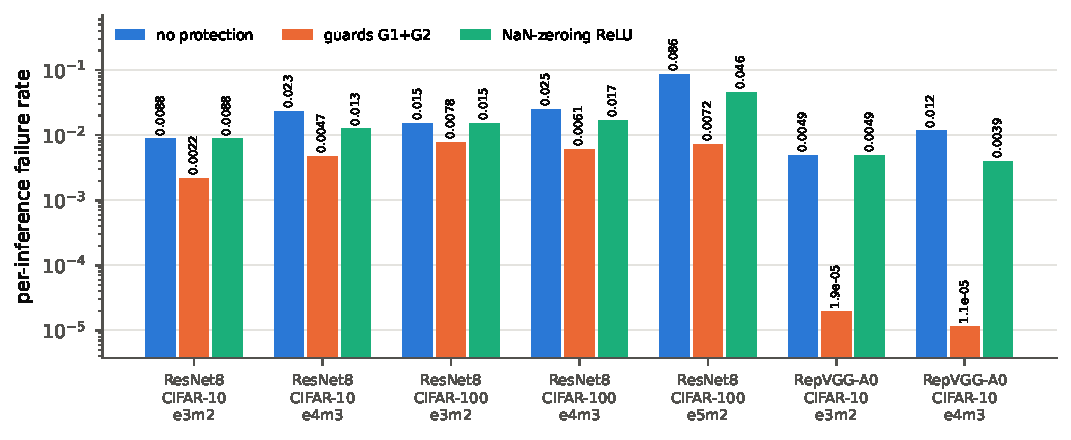
\includegraphics[width=\textwidth]{fig/e29_guards.pdf}
\caption{Per-inference failure rate on every network and format (log scale): with no protection,
with the read guards G1+G2, and with a NaN-zeroing ReLU instead.}
\label{fig:e29}
\end{figure}

\noindent The results confirm the algorithm on every network:
\begin{itemize}
    \item \textbf{Every catastrophic fault is $0\to1$}, in all 7 runs, as Proposition~1 says.
          $0\to1$ flips cause 77--100\% of all damage.
    \item \textbf{The catastrophic cases dominate, and more so on the larger network.} On
          RepVGG-A0 they are 0.5--1.2\% of faults but 88--95\% of damage, and the ordinary element
          cases did no measurable damage at all. A bigger network absorbs small errors, but not
          NaN, $\infty$ or a $2^{128}$ scale.
    \item \textbf{The guards carry over and help most where they are needed most.} G1+G2 cut the
          rate $4$--$12\times$ on ResNet8 and by two to three orders of magnitude on RepVGG-A0. The
          exception is ResNet8 on CIFAR-100 in \fmt{e3m2} ($1.9\times$). That network has low
          decision margins (55\% accuracy), so ordinary finite errors cause a larger share of the
          damage, and the guards do not target those.
    \item \textbf{The ReLU only helps formats that have NaN codes.} It changes nothing for
          \fmt{e3m2} (no NaN codes; S2 gives $+\infty$, which passes the ReLU), and helps
          $1.5$--$3\times$ for \fmt{e4m3} and \fmt{e5m2}. This is exactly what stage~3 predicts.
    \item \textbf{A catastrophic flip can be silent.} On RepVGG-A0 in \fmt{e3m2}, the S2 flips
          damage 87\% of predictions, but only 8\% of them give a non-finite output. The weight
          becomes huge but stays finite, because $|P_B|\,2^{128}$ does not overflow FP32 there
          (the stage-3 rule). An \texttt{isfinite} check on the output misses these, but the scale
          check D2 catches all of them.
\end{itemize}

\subsection{Interpretation}

\begin{enumerate}
    \item \textbf{Most failures come from a tiny, exactly known set of bits.} The catastrophic
          cases are 1--2\% of storage and are found by counting, not by injection.
    \item \textbf{The case tree is enough for the catastrophic part, but not for small errors.}
          For those, the size of the error reaching the next layer is what matters.
    \item \textbf{Every catastrophic flip is $0\to1$.} The direction of memory upsets changes
          the failure rate by $7$--$8\times$, so it belongs in the fault model.
    \item \textbf{Protection should follow the case, not the bit position.} In \fmt{e3m2}, scale
          bit 7 alone is 0.5\% of storage and 57\% of damage, so protecting a few bits works. In
          \fmt{e4m3}, NaN damage is spread over every element bit and 27\% of storage is needed for
          half the damage; the free guards G1+G2 do far better at zero storage cost.
    \item \textbf{The algorithm is cheap to use and carries over.} Counting cases needs no
          injection, and a campaign planned by case needs about a thousand injections instead of
          hundreds of thousands. Its predictions held on a larger network and a harder dataset,
          where the catastrophic cases matter even more.
\end{enumerate}

% ═════════════════════════════════════════════════════════════════════════════
\section{Conclusion}
% ═════════════════════════════════════════════════════════════════════════════

This phase of the project turned a fault-injection study of MX networks into an algorithm that
says, for every single-bit flip, what it will do and why. The algorithm follows a flip through
five stages (fault model, encoding, read checks, datapath, decision), and its core case tree puts
every flip into exactly one of 22 cases, which was verified by exhaustive enumeration over five
formats.

Measured against 1.1 million exhaustive injections, the case explains 91--97\% of the variance in
damage. Three catastrophic cases, 1--2\% of all bits, cause more than half of all failures, and
all of them are $0\to1$ flips. Two read-time guards that follow from the algorithm cut the
failure rate $4.3$--$5.2\times$ with no extra memory, and a NaN-zeroing ReLU makes a NaN weight
almost harmless.

Used as a campaign plan, the algorithm reproduced the exhaustive ResNet8 rates with about 1,000
injections. On a CIFAR-100 ResNet8 and a 7-million-parameter RepVGG-A0, every prediction held:
all catastrophic flips were $0\to1$, the catastrophic cases carried 33--95\% of the damage, and
the free guards cut the failure rate by $1.9\times$ to more than $250\times$. The practical
message is simple: in an MX network, protect the few flips the algorithm names, mainly scale
overflows and flips into NaN codes, and the rest matters far less.

% ═════════════════════════════════════════════════════════════════════════════
\section{Future Work}
% ═════════════════════════════════════════════════════════════════════════════

\begin{itemize}
    \item \textbf{Faults outside stored MX values.} Accumulators, partial sums, biases,
          normalisation parameters and address logic are not covered yet.
    \item \textbf{Accumulating faults.} Weight faults are persistent and can pile up between
          reloads; only single faults and pairs within one word were measured.
    \item \textbf{Other datapaths, measured end to end.} Saturating overflow, FP16
          accumulation and a full MX activation pipeline are stated as rules here, not injected.
    \item \textbf{Larger models and ImageNet.} DeiT and ImageNet were out of reach on the
          available hardware. The stratified plan of Section~\ref{sec:stratified} is what would
          make such a campaign affordable.
    \item \textbf{Hardware validation} of the guards G1 and G2 on an FPGA or accelerator model.
\end{itemize}

% ═════════════════════════════════════════════════════════════════════════════
\section*{Acknowledgements}
\addcontentsline{toc}{section}{Acknowledgements}

I thank my supervisor, \supervisor, for the problem statement and guidance throughout this
project, and IIT Kanpur for access to its GPU cluster.

% ═════════════════════════════════════════════════════════════════════════════
\begin{thebibliography}{99}
\addcontentsline{toc}{section}{References}

\bibitem{rouhani2023mx}
B.~D. Rouhani et al., ``Microscaling data formats for deep learning,''
\emph{arXiv:2310.10537}, 2023.

\bibitem{ocp2023mx}
Open Compute Project, ``OCP Microscaling Formats (MX) Specification, Version 1.0,'' 2023.

\bibitem{li2017understanding}
G.~Li, S.~K.~S. Hari, M.~Sullivan, T.~Tsai, K.~Pattabiraman, J.~Emer, and S.~W. Keckler,
``Understanding error propagation in deep learning neural network (DNN) accelerators and
applications,'' in \emph{Proc. SC}, 2017.

\bibitem{reagen2018ares}
B.~Reagen et al., ``Ares: A framework for quantifying the resilience of deep neural
networks,'' in \emph{Proc. DAC}, 2018.

\bibitem{mahmoud2020pytorchfi}
A.~Mahmoud et al., ``PyTorchFI: A runtime perturbation tool for DNNs,'' in \emph{Proc.
DSN Workshops}, 2020.

\bibitem{leveugle2009sfi}
R.~Leveugle, A.~Calvez, P.~Maistri, and P.~Vanhauwaert, ``Statistical fault injection:
Quantified error and confidence,'' in \emph{Proc. DATE}, 2009.

\bibitem{treefi2026}
TreeFI: value-aware statistical fault injection for DNNs, in \emph{Proc. ICCAD}, 2026.

\bibitem{rakin2019bfa}
A.~S. Rakin, Z.~He, and D.~Fan, ``Bit-flip attack: Crushing neural network with progressive
bit search,'' in \emph{Proc. ICCV}, 2019.

\bibitem{hong2019terminal}
S.~Hong, P.~Frigo, Y.~Kaya, C.~Giuffrida, and T.~Dumitra\c{s}, ``Terminal brain damage:
Exposing the graceless degradation in deep neural networks under hardware fault attacks,''
in \emph{Proc. USENIX Security}, 2019.

\bibitem{he2016resnet}
K.~He, X.~Zhang, S.~Ren, and J.~Sun, ``Deep residual learning for image recognition,'' in
\emph{Proc. CVPR}, 2016.

\bibitem{banbury2021mlperftiny}
C.~Banbury et al., ``MLPerf Tiny benchmark,'' in \emph{Proc. NeurIPS Datasets and
Benchmarks Track}, 2021.

\bibitem{ding2021repvgg}
X.~Ding, X.~Zhang, N.~Ma, J.~Han, G.~Ding, and J.~Sun, ``RepVGG: Making VGG-style ConvNets
great again,'' in \emph{Proc. CVPR}, 2021.

\end{thebibliography}

\end{document}
